\documentclass[aspectratio=169,11pt]{beamer}
\makeatletter
\def\input@path{{.}{docs/}{./docs/}{../docs/}}
\makeatother
% shared notation and packages for slides.tex and report.tex
\usepackage{amsmath,amssymb}
\usepackage{booktabs}
\usepackage{graphicx}
\usepackage{siunitx}
\usepackage{xcolor}
\usepackage{tikz}
\usetikzlibrary{arrows.meta,positioning,shapes.geometric,calc}
\makeatletter
\providecommand{\input@path}{}
\g@addto@macro\input@path{{.}{docs/}{./docs/}{../docs/}}
\makeatother
\graphicspath{{../figures/}{figures/}{docs/figures/}}
% generated by code/12_export_tex.py -- do not edit by hand
\newcommand{\VfourMaize}{0.018}
\newcommand{\VfourPwMaize}{0.005}
\newcommand{\VfourPwRice}{0.001}
\newcommand{\VfourPwSoybean}{0.009}
\newcommand{\VfourPwWheat}{0.084}
\newcommand{\VfourRice}{0.002}
\newcommand{\VfourSoybean}{0.008}
\newcommand{\VfourWheat}{0.065}
\newcommand{\adqYears}{2021--2023}
\newcommand{\bTMaizeSAfrica}{-27.8}
\newcommand{\bTMaizeUSA}{-6.4}
\newcommand{\bTRiceIndia}{-11.4}
\newcommand{\bTWheatIndia}{-4.2}
\newcommand{\bWMaizeSAfrica}{+0.0}
\newcommand{\bWMaizeUSA}{+0.0}
\newcommand{\bWRiceIndia}{+0.0}
\newcommand{\bWWheatIndia}{+0.0}
\newcommand{\bdRiceKcal}{63}
\newcommand{\bdRiceZinc}{55}
\newcommand{\bdShockKcal}{-6.3}
\newcommand{\bdShockKcalAbs}{6.3}
\newcommand{\bdShockMar}{-0.50}
\newcommand{\egWheatIron}{46}
\newcommand{\egWheatKcal}{34}
\newcommand{\egWheatSone}{-3.6}
\newcommand{\egWheatZinc}{48}
\newcommand{\exEheat}{1.00}
\newcommand{\exEwater}{0.33}
\newcommand{\exI}{0.222}
\newcommand{\exImax}{0.421}
\newcommand{\exIn}{0.53}
\newcommand{\exLheat}{0.58}
\newcommand{\exLwater}{17.8}
\newcommand{\exSheat}{0.43}
\newcommand{\exShlit}{0.50}
\newcommand{\exShobs}{0.36}
\newcommand{\exSwater}{0.44}
\newcommand{\exSwlit}{0.88}
\newcommand{\exSwobs}{0.00}
\newcommand{\exVfour}{0.151}
\newcommand{\feRatioBangladesh}{0.70}
\newcommand{\feRatioBrazil}{0.97}
\newcommand{\feRatioEgypt}{1.20}
\newcommand{\feRatioIndia}{0.89}
\newcommand{\feRatioNigeria}{0.91}
\newcommand{\feRatioRussia}{1.14}
\newcommand{\feRatioSAfrica}{0.82}
\newcommand{\heatCellsMaize}{7}
\newcommand{\heatCellsRice}{2}
\newcommand{\heatCellsSoybean}{0}
\newcommand{\heatCellsWheat}{22}
\newcommand{\inRiceSone}{-4.8}
\newcommand{\inWheatKcal}{-2.1}
\newcommand{\inWheatMar}{-0.52}
\newcommand{\inWheatMarTrade}{-0.28}
\newcommand{\koppenAgree}{93}
\newcommand{\koppenAgreeMaize}{92}
\newcommand{\koppenAgreeRice}{93}
\newcommand{\koppenAgreeSoybean}{95}
\newcommand{\koppenAgreeWheat}{83}
\newcommand{\maizeFeedBrazil}{75}
\newcommand{\maizeFeedChina}{72}
\newcommand{\maizeFeedUS}{46}
\newcommand{\maizeFeedWorld}{60}
\newcommand{\maizeFoodSAfrica}{40}
\newcommand{\maizeFoodWorld}{12}
\newcommand{\marBangladesh}{0.939}
\newcommand{\marBrazil}{0.994}
\newcommand{\marEgypt}{1.000}
\newcommand{\marIndia}{0.978}
\newcommand{\marNigeria}{0.981}
\newcommand{\marRussia}{1.000}
\newcommand{\marSAfrica}{0.964}
\newcommand{\mcFourMaizeFirst}{1.0}
\newcommand{\mcFourRiceFirst}{0.0}
\newcommand{\mcFourSoybeanFirst}{1.5}
\newcommand{\mcFourWheatFirst}{97.5}
\newcommand{\mcOneMaizeFirst}{1.0}
\newcommand{\mcOneRiceFirst}{0.0}
\newcommand{\mcOneSoybeanFirst}{1.3}
\newcommand{\mcOneWheatFirst}{97.7}
\newcommand{\nCountriesAdq}{205}
\newcommand{\nPassNew}{26}
\newcommand{\nPassNewSig}{1}
\newcommand{\nPassOld}{26}
\newcommand{\nPassOldSig}{9}
\newcommand{\nRobustT}{7}
\newcommand{\nRobustW}{5}
\newcommand{\nShared}{5}
\newcommand{\nShock}{26}
\newcommand{\orderFour}{Wheat $>$ Maize $>$ Soybean $>$ Rice}
\newcommand{\orderFourPw}{Wheat $>$ Soybean $>$ Maize $>$ Rice}
\newcommand{\orderOne}{Wheat $>$ Maize $>$ Soybean $>$ Rice}
\newcommand{\pShock}{0.170}
\newcommand{\pShockE}{0.169}
\newcommand{\pShockS}{0.467}
\newcommand{\panelShareMaize}{69}
\newcommand{\panelShareRice}{63}
\newcommand{\panelShareSoybean}{90}
\newcommand{\panelShareWheat}{51}
\newcommand{\passRiceBangladesh}{0.37}
\newcommand{\passRiceChina}{0.90}
\newcommand{\passRiceIndia}{0.37}
\newcommand{\passSoyHi}{1.8}
\newcommand{\passSoyLo}{1.6}
\newcommand{\poolTMaize}{-11.7}
\newcommand{\poolTRice}{-1.1}
\newcommand{\poolTSoybean}{-6.2}
\newcommand{\poolTWheat}{-2.7}
\newcommand{\poolTpMaize}{0.000}
\newcommand{\poolTpRice}{0.476}
\newcommand{\poolTpSoybean}{0.000}
\newcommand{\poolTpWheat}{0.019}
\newcommand{\poolWMaize}{+1.5}
\newcommand{\poolWRice}{+0.3}
\newcommand{\poolWSoybean}{+1.8}
\newcommand{\poolWWheat}{-2.4}
\newcommand{\poolWpMaize}{0.079}
\newcommand{\poolWpRice}{0.422}
\newcommand{\poolWpSoybean}{0.020}
\newcommand{\poolWpWheat}{0.080}
\newcommand{\pshareIronMaize}{8.3}
\newcommand{\pshareIronRice}{9.4}
\newcommand{\pshareIronSoybean}{1.2}
\newcommand{\pshareIronWheat}{32.8}
\newcommand{\pshareProteinMaize}{5.1}
\newcommand{\pshareProteinRice}{13.4}
\newcommand{\pshareProteinSoybean}{0.6}
\newcommand{\pshareProteinWheat}{21.9}
\newcommand{\pshareZincMaize}{7.6}
\newcommand{\pshareZincRice}{15.3}
\newcommand{\pshareZincSoybean}{0.5}
\newcommand{\pshareZincWheat}{32.5}
\newcommand{\rankFourMaize}{2}
\newcommand{\rankFourPwMaize}{3}
\newcommand{\rankFourPwRice}{4}
\newcommand{\rankFourPwSoybean}{2}
\newcommand{\rankFourPwWheat}{1}
\newcommand{\rankFourRice}{4}
\newcommand{\rankFourSoybean}{3}
\newcommand{\rankFourWheat}{1}
\newcommand{\rhoShock}{+0.20}
\newcommand{\rhoShockE}{+0.19}
\newcommand{\rhoShockS}{+0.02}
\newcommand{\rhoZhaoClim}{+0.8}
\newcommand{\rhoZhaoFour}{+0.6}
\newcommand{\rhoZhaoFourPw}{+0.0}
\newcommand{\rhoZhaoHeat}{+0.8}
\newcommand{\rhoZhaoOne}{+0.6}
\newcommand{\rhoZhaoPool}{+0.4}
\newcommand{\riskIronMaize}{0.48}
\newcommand{\riskIronRice}{0.49}
\newcommand{\riskIronSoybean}{0.05}
\newcommand{\riskIronWheat}{1.67}
\newcommand{\riskProteinMaize}{0.00}
\newcommand{\riskProteinRice}{1.05}
\newcommand{\riskProteinSoybean}{0.00}
\newcommand{\riskProteinWheat}{1.38}
\newcommand{\riskZincMaize}{0.00}
\newcommand{\riskZincRice}{0.51}
\newcommand{\riskZincSoybean}{0.02}
\newcommand{\riskZincWheat}{3.02}
\newcommand{\robN}{80}
\newcommand{\robWheatTopAll}{80}
\newcommand{\rtwoMaize}{0.24}
\newcommand{\rtwoMaxMaize}{0.50}
\newcommand{\rtwoMaxRice}{0.26}
\newcommand{\rtwoMaxSoybean}{0.54}
\newcommand{\rtwoMaxWheat}{0.22}
\newcommand{\rtwoMinMaize}{0.05}
\newcommand{\rtwoMinRice}{0.01}
\newcommand{\rtwoMinSoybean}{0.05}
\newcommand{\rtwoMinWheat}{0.02}
\newcommand{\rtwoRice}{0.04}
\newcommand{\rtwoSoybean}{0.17}
\newcommand{\rtwoWheat}{0.13}
\newcommand{\saMaizeSone}{-26.8}
\newcommand{\sharedPanel}{Brazil, China, India, Russia, USA}
\newcommand{\sharedWheatTop}{5}
\newcommand{\skillMedian}{0.31}
\newcommand{\skillN}{21}
\newcommand{\skillPos}{18}
\newcommand{\snrHeatMaize}{0.68}
\newcommand{\snrHeatRice}{0.92}
\newcommand{\snrHeatSoybean}{0.64}
\newcommand{\snrHeatWheat}{0.80}
\newcommand{\soyFoodWorld}{4}
\newcommand{\soyProcChina}{81}
\newcommand{\soyProcUS}{92}
\newcommand{\soyProcWorld}{86}
\newcommand{\tauOneFour}{0.91}
\newcommand{\tauOneThree}{0.58}
\newcommand{\worldFatMaize}{1.4}
\newcommand{\worldFatRice}{1.8}
\newcommand{\worldFatSoybean}{12.5}
\newcommand{\worldFatWheat}{3.5}
\newcommand{\worldIMaize}{4.2}
\newcommand{\worldIRice}{10.2}
\newcommand{\worldISoybean}{4.5}
\newcommand{\worldIWheat}{18.7}
\newcommand{\worldIronMaize}{5.6}
\newcommand{\worldIronRice}{7.6}
\newcommand{\worldIronSoybean}{3.3}
\newcommand{\worldIronWheat}{26.0}
\newcommand{\worldKcalMaize}{4.9}
\newcommand{\worldKcalRice}{17.1}
\newcommand{\worldKcalSoybean}{3.7}
\newcommand{\worldKcalWheat}{17.8}
\newcommand{\worldProteinMaize}{3.3}
\newcommand{\worldProteinRice}{11.4}
\newcommand{\worldProteinSoybean}{1.8}
\newcommand{\worldProteinWheat}{18.8}
\newcommand{\worldZincMaize}{5.8}
\newcommand{\worldZincRice}{13.1}
\newcommand{\worldZincSoybean}{1.3}
\newcommand{\worldZincWheat}{27.2}
\newcommand{\worstMar}{-0.53}
\newcommand{\worstMarCase}{Maize in S. Africa}



\definecolor{rice}{HTML}{2A7F62}
\definecolor{wheat}{HTML}{C8961A}
\definecolor{maize}{HTML}{C0504D}
\definecolor{soy}{HTML}{5B5EA6}
\definecolor{ink}{HTML}{222222}
\definecolor{muted}{HTML}{6B6B6B}
\definecolor{paddy}{HTML}{1F4E3D}
\definecolor{grain}{HTML}{C8961A}
\definecolor{clay}{HTML}{B5523B}
\newcommand{\Teff}{T_{\mathrm{eff}}}
\newcommand{\Tcrit}{T_{\mathrm{crit}}}
\newcommand{\ETc}{\mathrm{ET_c}}
\newcommand{\ETo}{\mathrm{ET_0}}
\usepackage{adjustbox}


\usepackage[round]{natbib}
\usepackage{booktabs}
\bibliographystyle{plainnat}
\let\parencite\citep
\let\textcite\citet
\hypersetup{colorlinks=true,linkcolor=paddy,citecolor=paddy,urlcolor=paddy}

% ---------------- look ----------------
\usetheme{default}
\usecolortheme{default}
\setbeamercolor{structure}{fg=paddy}
\setbeamercolor{frametitle}{fg=paddy}
\setbeamercolor{title}{fg=paddy}
\setbeamercolor{alerted text}{fg=clay}
\setbeamercolor{block title}{bg=paddy,fg=white}
\setbeamercolor{block body}{bg=paddy!6}
\setbeamercolor{block title alerted}{bg=clay,fg=white}
\setbeamercolor{block body alerted}{bg=clay!7}
\setbeamerfont{frametitle}{series=\bfseries,size=\large}
\setbeamertemplate{navigation symbols}{}
\setbeamertemplate{itemize items}[circle]
\setbeamertemplate{footline}{\hfill{\scriptsize\color{muted}\insertsection\quad\insertframenumber\,/\,\inserttotalframenumber}\hspace*{1em}\vspace*{0.6em}}
\setbeamertemplate{frametitle}{\vspace*{0.4em}\insertframetitle\par\vspace*{-0.2em}{\color{grain}\rule{2.2em}{2pt}}}
\newcommand{\cropdot}[1]{\textcolor{#1}{\rule{0.7em}{0.7em}}}
\setlength{\abovedisplayskip}{1pt}\setlength{\belowdisplayskip}{1pt}\setlength{\abovedisplayshortskip}{1pt}\setlength{\belowdisplayshortskip}{1pt}
\newcommand{\TT}{\mathrm{T}}   % temperature
\newcommand{\PP}{\mathrm{P}}   % precipitation

\title{Climate Change and Nutritional Security:\\[0.2em] Which Crops Are Most Vulnerable?}
\subtitle{A Climate-Nutrition Vulnerability Index for rice, wheat, maize and soybean}
\author{Arpit Mahtele \and Dev Patel \and Navey Puri \and Shreyash Lohare}
\date{Earth 616}

\begin{document}

\begin{frame}[plain]
\titlepage
\vspace{-1.2em}
\begin{center}\scriptsize\color{muted}
\cropdot{rice} rice\quad \cropdot{wheat} wheat\quad \cropdot{maize} maize\quad \cropdot{soy} soybean
\end{center}
\end{frame}

% =====================================================================
% \section{Problem}
\begin{frame}{Problem and research gap}
\begin{columns}[T]
\column{0.52\textwidth}\small
\begin{itemize}
\item Studies measure climate's effect on \emph{yield} \parencite{ray2015,zhao2017} and CO$_2$'s effect on \emph{nutrients} \parencite{myers2014,smith2018} separately.
\item Their scores are on different scales, so crops cannot be ranked together.
\end{itemize}
\begin{alertblock}{Gap (from our literature review)}
No study combines climatic \textbf{exposure}, crop \textbf{sensitivity} and \textbf{nutritional importance} in one index.
\end{alertblock}
\column{0.44\textwidth}\small
\textbf{Our questions}
\begin{enumerate}
\item Which crop is most vulnerable to observed temperature and precipitation change based on its nutrional importance?
\item If a crop's yield falls, what happens to a country's nutrient supply?
\end{enumerate}
\end{columns}
\end{frame}

\begin{frame}{Countries analysed}
\vspace*{-1.0em}
\begin{columns}[onlytextwidth,c]
\column{0.48\textwidth}\footnotesize
\textbullet\ \textbf{Core:} USA, Brazil, India, China, Russia.
\column{0.52\textwidth}\footnotesize
\textbullet\ \textbf{Others:} Top producers in different climate zones.
\end{columns}
\vspace{0.1em}
\centering
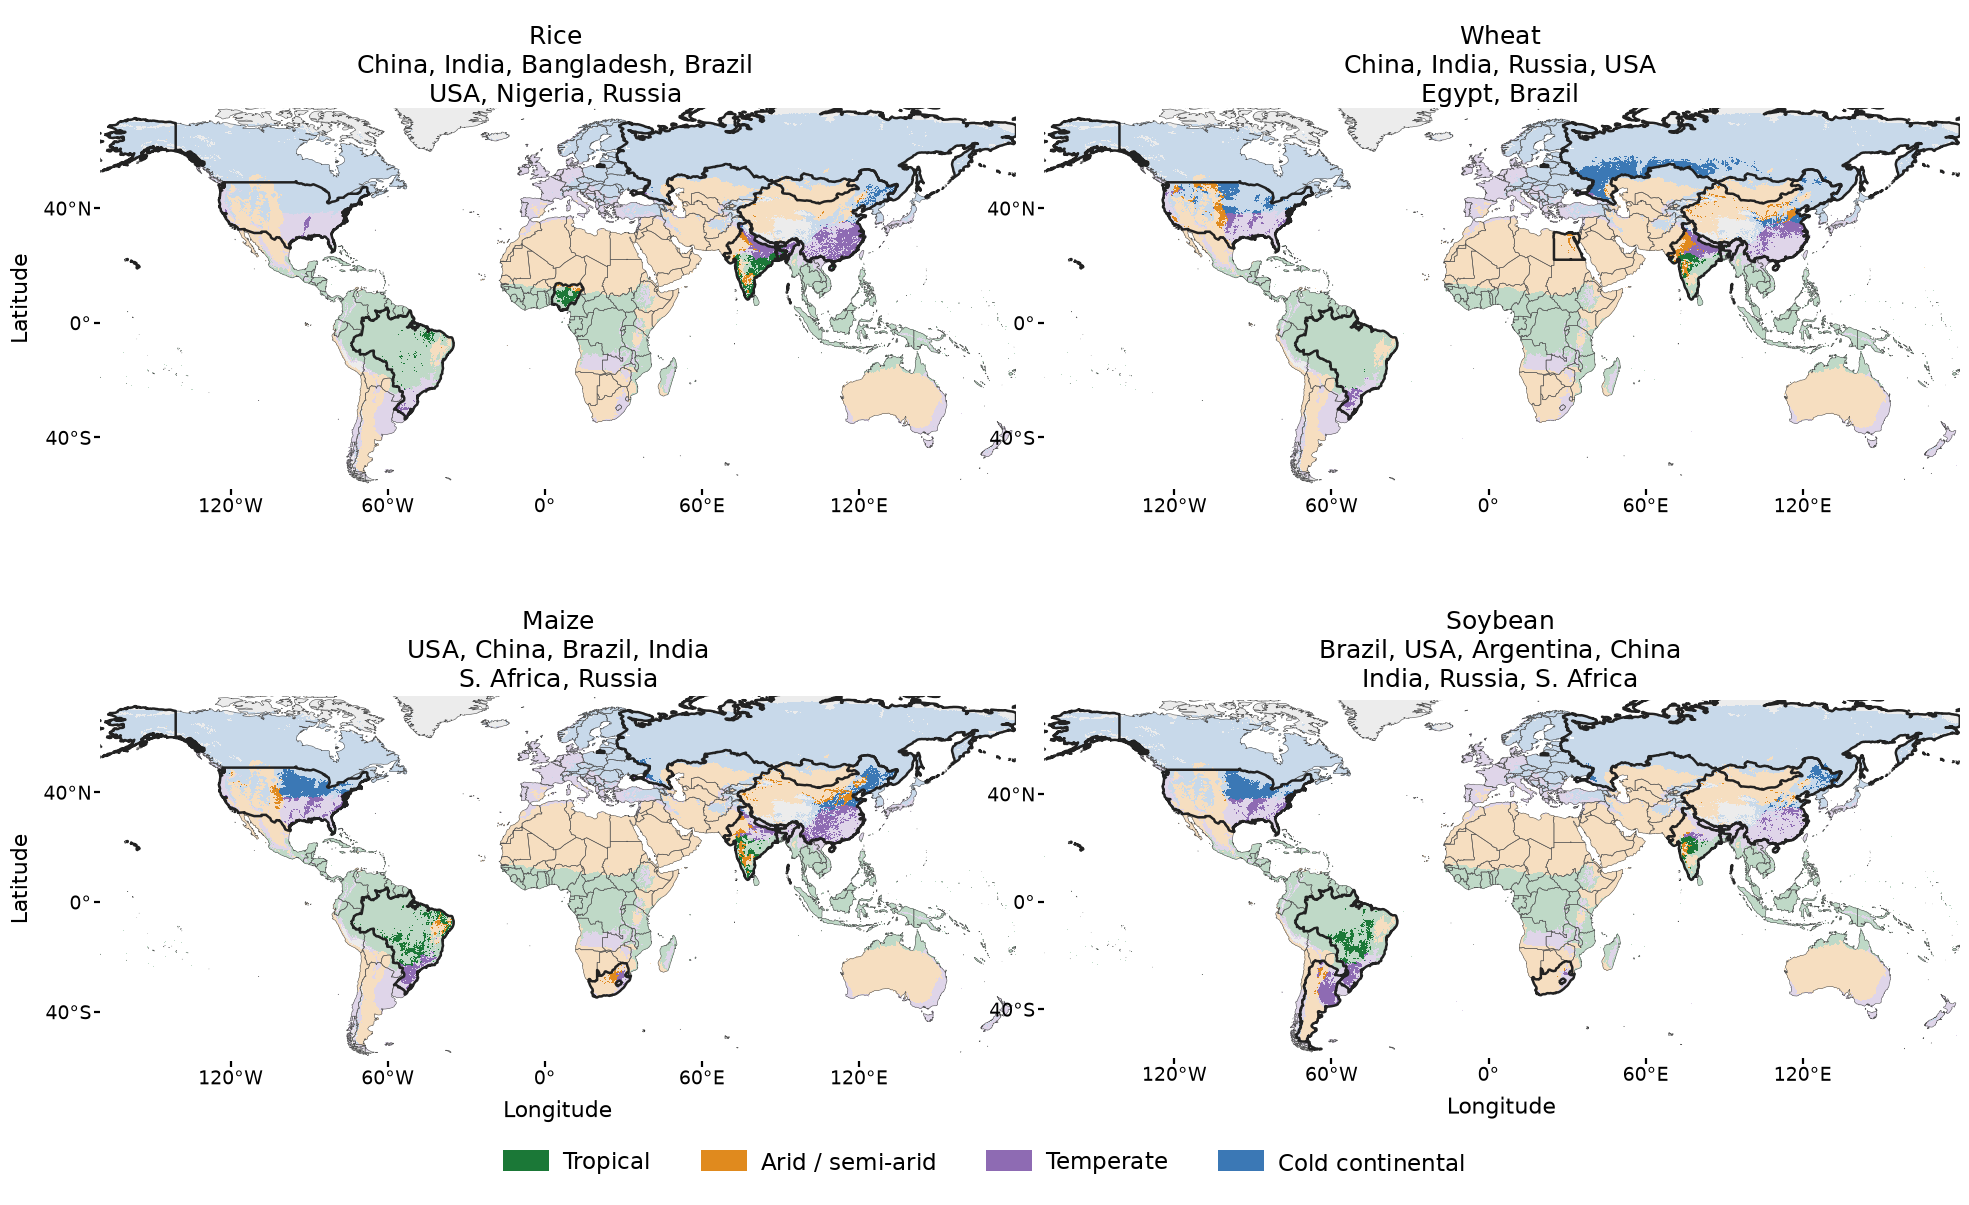
\includegraphics[width=0.92\linewidth,height=0.78\textheight,keepaspectratio]{F01_panels_koppen.png}
\end{frame}

% =====================================================================
% \section{Method}
\begin{frame}{Framework: Vulnerability = Exposure $\times$ Sensitivity $\times$ Importance}
\centering
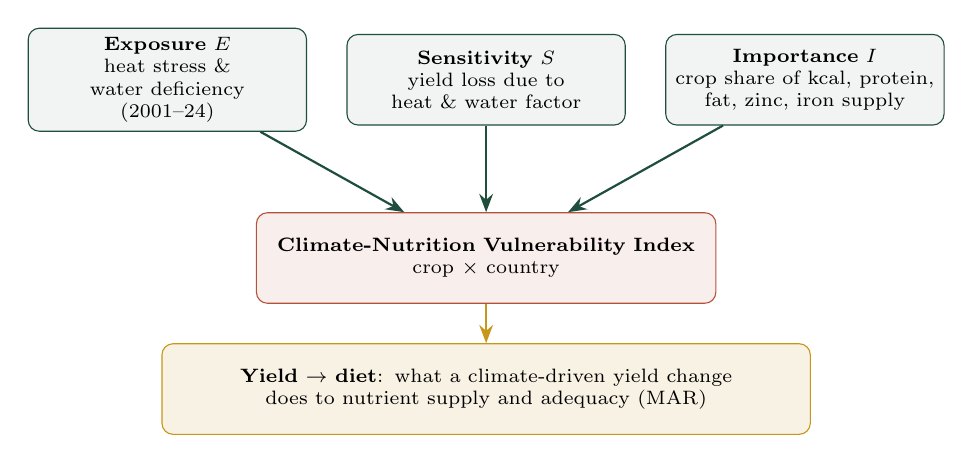
\begin{tikzpicture}[node distance=0.5cm and 0.5cm, box/.style={draw=paddy,fill=paddy!6,rounded corners,align=center,font=\scriptsize,minimum height=1.15cm,text width=3.3cm}, arr/.style={-Stealth,thick,paddy}]
\node[box] (E) {\textbf{Exposure $E$}\\ heat stress \&\\ water deficiency \\ (2001--24)};
\node[box,right=of E] (S) {\textbf{Sensitivity $S$}\\ yield loss due to \\ heat \& water factor};
\node[box,right=of S] (I) {\textbf{Importance $I$}\\ crop share of kcal, protein,\\ fat, zinc, iron supply};
\node[box,below=1.1cm of S,fill=clay!10,draw=clay,text width=5.6cm] (V) {\textbf{Climate-Nutrition Vulnerability Index}\\ crop $\times$ country};
\draw[arr] (E) -- (V); \draw[arr] (S) -- (V); \draw[arr] (I) -- (V);
\node[box,below=0.5cm of V,fill=grain!12,draw=grain,text width=8cm] (D) {\textbf{Yield $\rightarrow$ diet}: what a climate-driven yield change does to nutrient supply and adequacy (MAR)};
\draw[arr,grain] (V) -- (D);
\end{tikzpicture}
\par\vspace{0.5em}\scriptsize
IPCC-style framing with \emph{Adaptive capacity} replaced by \emph{Importance}.
\end{frame}

\begin{frame}{Our formula for the Index}
\footnotesize
\begin{tabular}{p{1.2cm}p{3.4cm}p{8.0cm}}
\toprule
 & Formula & Verdict\\
\midrule
F1 & $E\cdot S\cdot I$ & \textcolor{clay}{Rejected}: lets heat exposure multiply water sensitivity\\
F2 & $(E\,S\,I)^{1/3}$ & \textcolor{clay}{Rejected}: same ranking as F1, only rescaled\\
F3 & $(E+S+I)/3$ & \textcolor{clay}{Rejected}: high exposure can make up for a crop nobody eats\\
\textbf{F4} & $\tfrac12(E^{\TT}S^{\TT}+E^{\PP}S^{\PP})\,I$ & \textcolor{paddy}{\textbf{Chosen}}: each stress meets its own sensitivity; zero if nobody eats the crop\\
\bottomrule
\end{tabular}
\par\vspace{0.5em}\scriptsize The choice rests on these design reasons; calculations show that there is not much variance in the ordering of vulnerability score.
\end{frame}

\begin{frame}{Exposure to temperature (heat)}
\begin{block}{Formula}
\[E^{\TT}=\frac{L^{\TT}}{\max L^{\TT}},\qquad L^{\TT}=\operatorname*{mean}_{2001\text{--}24}\ \frac{\sum_m w_m\,\max\!\big(0,\;T_{eff,m}-T_{crit}\big)}{\sum_m w_m}\]
\end{block}
\textbf{In words:} the average number of \si{\celsius} by which flowering-season temperature is above the crop's heat limit; then divided by the largest value among all crop-country pairs, so everything sits on 0--1.

\begin{columns}[T]
\column{0.55\textwidth}
\footnotesize
\begin{itemize}\setlength{\itemsep}{2pt}
\item $m$: month; $w_m$: share of month $m$ inside the flowering window (45--70\% of the season, \cite{deryng2014})
\item $T_{eff}=\tfrac12(T_{mean}+T_{max})$: effective temperature
\item $T_{crit}$: heat limit above which flowering is damaged
\end{itemize}
\column{0.42\textwidth}
\footnotesize
\begin{tabular}{@{}lc@{}}
\toprule
Crop & $T_{crit}$\\
\midrule
Rice & \SI{35}{\celsius}\\
Wheat & \SI{25}{\celsius}\\
Maize & \SI{32}{\celsius}\\
Soybean & \SI{35}{\celsius}\\
\bottomrule
\end{tabular}\\[0.3em]
Deryng 2014; rice: Yoshida 1981.\\[0.3em]
% \textbf{Example, wheat in India:} \exLheat\,\si{\celsius} above the limit (the largest of any pair), so $E^{\TT}=\exEheat$. \textbf{Limit:} monthly data hide hot days, so most rice and soybean pairs score zero.
\end{columns}
\end{frame}

\begin{frame}{Exposure to precipitation (water)}
\begin{block}{Formula}
\[E^{\PP}=\frac{L^{\PP}}{\max L^{\PP}},\qquad L^{\PP}=\operatorname*{mean}_{2001\text{--}24}\ \frac{\sum R\;\max\!\big(0,\;1-P/ET_c\big)}{\sum A}\]
\end{block}
\textbf{In words:} the share of the crop's water need that rain does not supply, counted on rainfed land; then divided by the largest value among all pairs (0--1).

\begin{columns}[T]
\column{0.55\textwidth}
\footnotesize
\begin{itemize}\setlength{\itemsep}{2pt}
\item $P$: rainfall in the growing season
\item $ET_c$: the crop's water need. \parencite{fao56}
\item $1-P/ET_c$: the shortfall (0 if rain is enough)
\item $R$: rainfed hectares, $A$: all hectares. Irrigated land counts as no shortfall
\end{itemize}
\column{0.42\textwidth}
\footnotesize
% \textbf{Example, wheat in India:} \exLwater\% of the water need is unmet on the rainfed part, so $E^{\PP}=\exEwater$.\\[0.4em]
\textbf{Why this form:} it is FAO's own idea (a crop's yield loss follows its water deficit \parencite{fao66}) computed from monthly rainfall and temperature, so it also runs on future climate data.\\[0.4em]
% \textbf{Limit:} simple water balance (no soil storage or canal irrigation).
\end{columns}
\end{frame}

\begin{frame}{Sensitivity to temperature (heat)}
\begin{block}{Formula}
\[S^{\TT}=\frac{s^{\TT}}{\max s^{\TT}},\qquad s^{\TT}=\frac{1}{T_{lim}-T_{crit}}\]
\end{block}
\textbf{In words:} fraction of yield lost per \si{\celsius} above the crop's heat limit, divided by the largest of the four crops (0--1).

\begin{columns}[T]
\column{0.52\textwidth}
\footnotesize
\begin{itemize}\setlength{\itemsep}{1pt}
\item $T_{crit}$: heat limit, where damage starts (same as in exposure)
\item $T_{lim}$: total loss; linear in between \parencite{deryng2014}
\end{itemize}
\textbf{Why it fits:} exposure = degrees above the limit; sensitivity = yield lost per degree above the limit; the product is the fraction of yield at risk.
\column{0.46\textwidth}
\footnotesize\centering
\adjustbox{max width=\linewidth}{\begin{tabular}{lcccc}
\toprule
Crop & $T_{crit}$ & $T_{lim}$ & loss per \si{\celsius} (\%) & $S^{T}$\\
\midrule
Rice & 35 & -- & 7.0 & 0.35 \\
Wheat & 25 & 35 & 10.0 & 0.50 \\
Maize & 32 & 45 & 7.7 & 0.38 \\
Soybean & 35 & 40 & 20.0 & 1.00 \\
\bottomrule
\end{tabular}
}\\[0.4em]
\end{columns}
\end{frame}

\begin{frame}{Sensitivity to precipitation (water)}
\begin{block}{Formula}
\[S^{\PP}=\frac{K_y}{\max K_y}\]
\end{block}
\textbf{In words:} FAO's water factor $K_y$: yield lost per unit of water shortfall, divided by the largest crop value (0--1).

\begin{columns}[T]
\column{0.52\textwidth}
\footnotesize
\begin{itemize}\setlength{\itemsep}{2pt}
\item FAO \parencite{fao66}: yield loss $=K_y\times$ water deficit; $K_y=1.25$: a 10\% shortfall costs about 12.5\% of yield
\item Same quantity as exposure (the unmet share of water need), so the two multiply cleanly
\end{itemize}
% \textbf{Example, wheat in India:} $E^{\PP}=\exEwater$, $S^{\PP}=\exSwlit$.
\column{0.46\textwidth}
\footnotesize\centering
\adjustbox{max width=\linewidth}{\begin{tabular}{lcc}
\toprule
Crop & $K_y$ & $S^{P}$\\
\midrule
Rice & 1.25 & 1.00 \\
Wheat & 1.10 & 0.88 \\
Maize & 1.25 & 1.00 \\
Soybean & 0.85 & 0.68 \\
\bottomrule
\end{tabular}
}\\[0.4em]
% \raggedright\scriptsize $^{\dagger}$ Rice has no FAO $K_y$; maize value (1.25) used as lower bound.
% \textbf{Limit:} $P/ET_c$ is a simple stand-in for FAO's evapotranspiration ratio.
\end{columns}
\end{frame}

\begin{frame}{Importance: how much do people depend on the crop?}
\begin{columns}[T]
\column{0.54\textwidth}
\begin{block}{Importance of a crop in a country}
\[ I=\frac15\Big(\text{share of kcal}+\text{protein}+\text{fat}+\text{zinc}+\text{iron}\Big) \]
\centering\small share = amount supplied by the crop $\big/$ total supply (2021--23)
\end{block}
\footnotesize
Data: FAO Food Balance Sheets; zinc and iron = food quantity $\times$ USDA content. Example: rice gives Bangladesh \bdRiceKcal\% of its calories and \bdRiceZinc\% of its zinc.
\column{0.42\textwidth}
\footnotesize
\textbf{Why an average?}
\begin{itemize}
    \item Nothing ranks calories above zinc, so equal weights are neutral
    \item An average lets a crop count where it is strong (soybean: \worldFatSoybean\% of world fat, \worldZincSoybean\% of zinc)
    \item A geometric mean would punish it for its weakest nutrient.
\end{itemize}
\end{columns}
\end{frame}

\begin{frame}{From yield to diet}
\begin{columns}[T]
\column{0.48\textwidth}
\begin{block}{1. History: pass-through}
\[\Delta\%\,\text{food supply}_t=a+\beta\,\Delta\%\,\text{yield}_t+\varepsilon_t\]
\end{block}
\footnotesize
\begin{itemize}\setlength{\itemsep}{1pt}
\item Take yield and food supply as \% above or below their long-term trend
\item $\beta=1$: food supply falls as much as yield
\item $\beta\approx0$: trade or stocks cover the gap
\item Shows a link, not a cause
\end{itemize}
\column{0.50\textwidth}
\begin{block}{2. What-if: yield falls 10\%}
\[f=|\Delta Y|\min(1,\mathrm{SSR}),\quad S'_n=S_n-f\,C_n\]
\end{block}
\footnotesize
\begin{itemize}\setlength{\itemsep}{1pt}
\item Suppose yield falls 10\%
\item $\mathrm{SSR}$ = own production $\div$ domestic supply
\item The crop loses a share $f$ of its calories, protein, fat, Zn and Fe ($C_n$ = what the crop supplies)
\item MAR is recomputed ($R_n$ = requirement); 1 = all needs met
\item No market response: prices, trade and stocks stay fixed; other foods unchanged
\end{itemize}
\end{columns}
\end{frame}

\begin{frame}{Scenario: from a yield loss to nutritional adequacy}
\footnotesize\setlength{\abovedisplayskip}{1pt}\setlength{\belowdisplayskip}{1pt}
\textbf{Assumption:} we do not model market responses. We assume no change in prices, trade, imports, exports or stocks after a yield shock, and other foods remain unchanged.
\begin{columns}[T]
\column{0.49\textwidth}
\textbf{1. Yield shock $\rightarrow$ food-supply loss}
\[f=|\Delta Y|\,\min(1,\mathrm{SSR})\]
\[\mathrm{SSR}=\frac{\text{domestic production}}{\text{domestic food supply}}\]
\begin{itemize}\setlength{\itemsep}{0pt}
\item $\Delta Y$ = \% change in yield; SSR = self-sufficiency ratio (baseline data); $\min(1,\mathrm{SSR})$ caps the factor at 1
\item \textbf{Example:} $\Delta Y=-10\%$, $\mathrm{SSR}=0.8$: $f=0.10\times0.8=0.08$, i.e.\ \fbox{8\% food-supply loss}
\end{itemize}
\vspace{0.3em}
\fbox{\parbox{0.92\linewidth}{\centering\scriptsize Yield loss $\rightarrow$ food-supply loss $\rightarrow$ nutrient loss $\rightarrow$ lower NAR $\rightarrow$ lower MAR}}
\column{0.49\textwidth}
\textbf{2. Loss $\rightarrow$ nutrients}
\[\boxed{S'_n=S_n-fC_n}\]
$S_n$ = national supply of nutrient $n$; $C_n$ = supplied by the crop; $S'_n$ = after the shock. The same fraction $f$ of the crop's kcal, protein, fat, Zn and Fe is removed.\par\vspace{0.3em}
\textbf{3. Recalculate adequacy}
\[\mathrm{NAR}_n=\min\!\Big(1,\frac{S'_n}{R_n}\Big),\quad \boxed{\mathrm{MAR}=\tfrac15\textstyle\sum_{n}\mathrm{NAR}_n}\]
\begin{itemize}\setlength{\itemsep}{0pt}
\item $R_n$ = requirement; $n\in\{$kcal, protein, fat, Zn, Fe$\}$
\item $\mathrm{NAR}_n$ capped at 1: a surplus of one nutrient cannot offset a deficiency of another
\item $\mathrm{MAR}=1$: all five requirements met
\end{itemize}
\end{columns}
\end{frame}

% =====================================================================
% \section{Results}
\begin{frame}{Heat stress where each crop grows}
\vspace*{-0.5em}
\centering
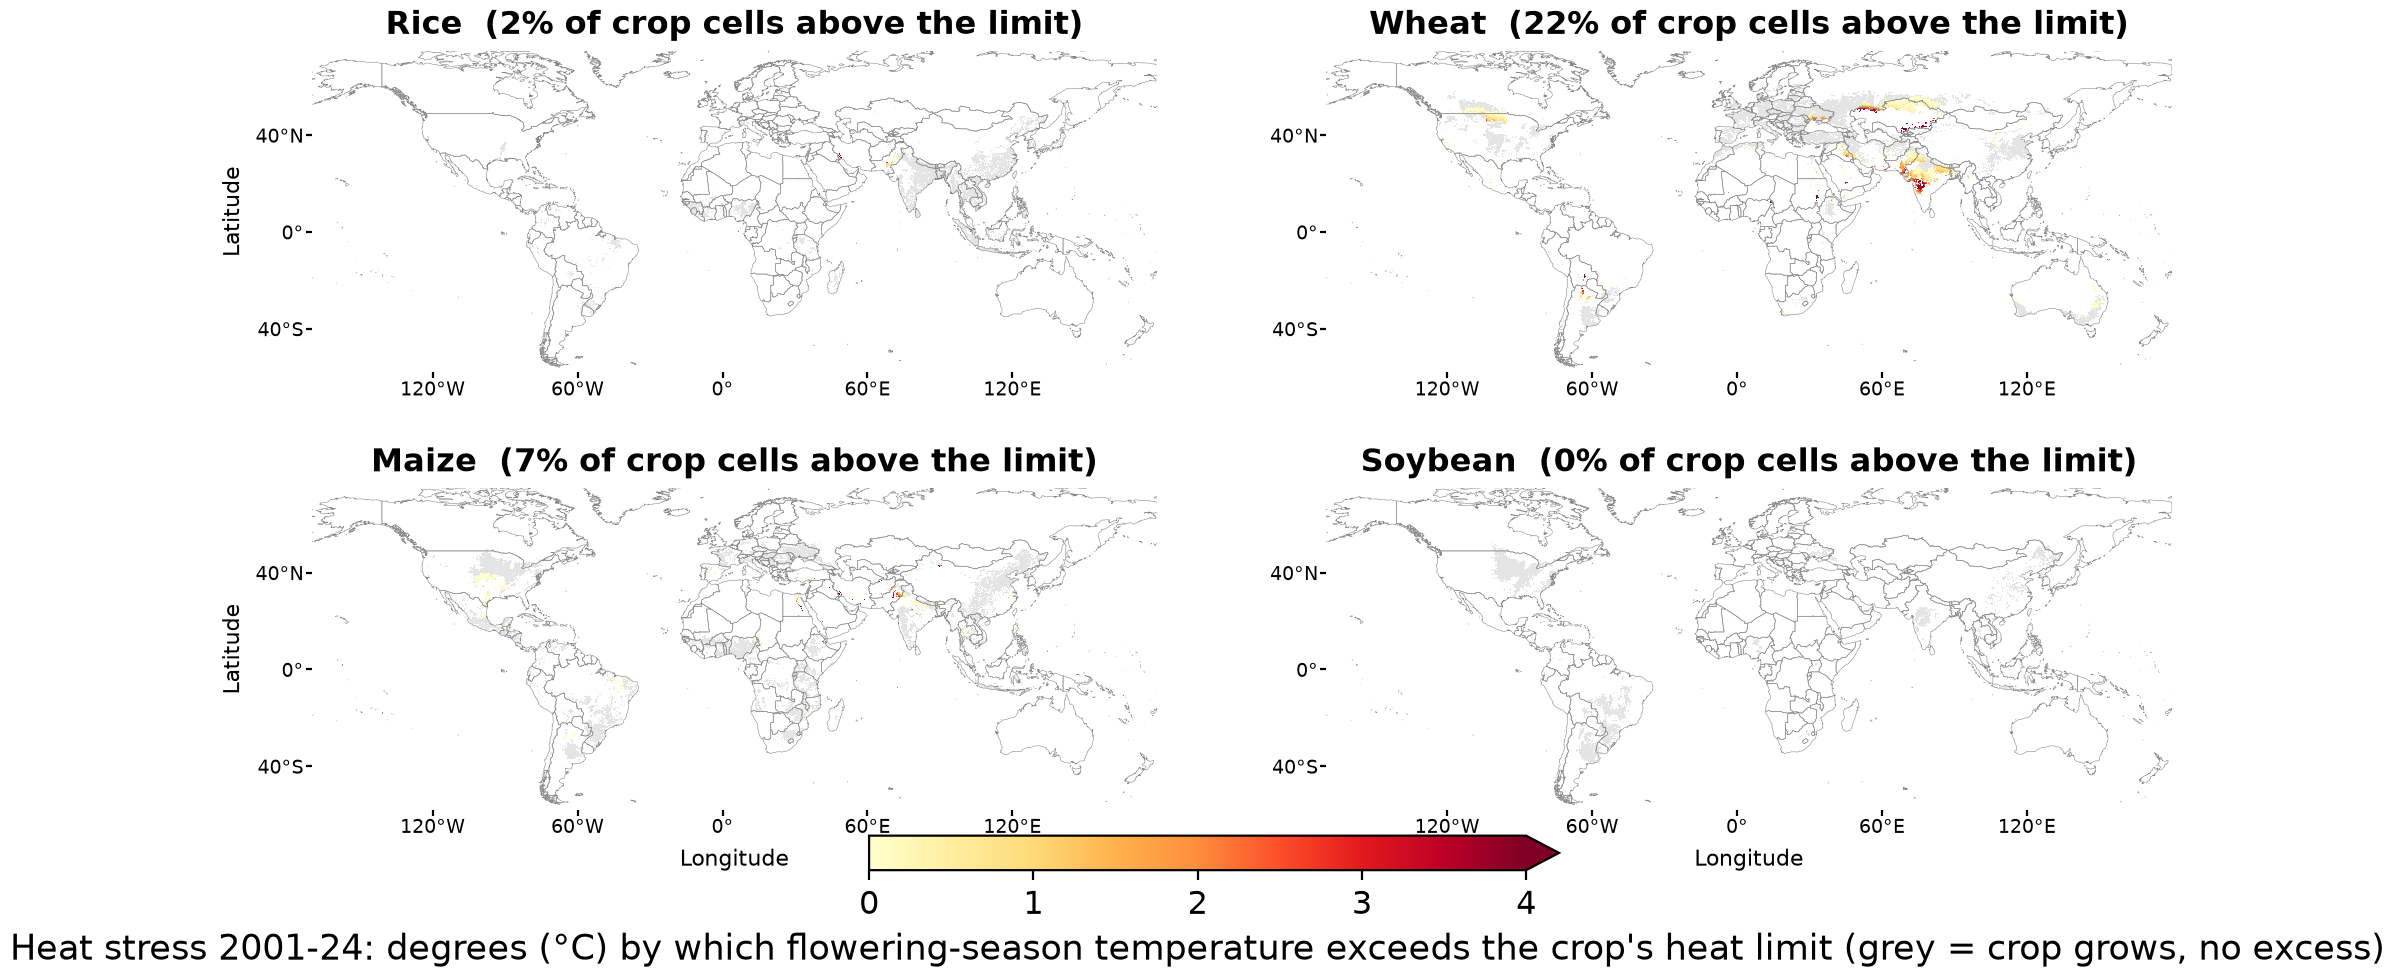
\includegraphics[width=0.98\linewidth,height=0.55\textheight,keepaspectratio]{F02c_heat_stress_map.png}
\vspace*{0.2em}

\begin{columns}[T,onlytextwidth]
\column{0.36\textwidth}
\scriptsize
\textbf{What we measure:}\\
Flowering-season temperature excess above crop heat limit $T_{crit}$ (2001--24 mean). Heat damage concentrates during flowering.
\column{0.28\textwidth}
\scriptsize\centering
\begin{tabular}{@{}lcc@{}}
\toprule
Crop & Limit & Cells above\\
\midrule
Rice & \SI{35}{\celsius} & \heatCellsRice\%\\
Wheat & \SI{25}{\celsius} & \heatCellsWheat\%\\
Maize & \SI{32}{\celsius} & \heatCellsMaize\%\\
Soybean & \SI{35}{\celsius} & \heatCellsSoybean\%\\
\bottomrule
\end{tabular}
\column{0.34\textwidth}
\scriptsize
\textbf{Main finding:}\\
\textbf{Wheat} is the most heat-exposed globally, largely because its threshold (\SI{25}{\celsius}) is much lower than other crops.
\end{columns}
\end{frame}

\begin{frame}{Water stress where each crop grows}
\vspace*{-0.5em}
\centering
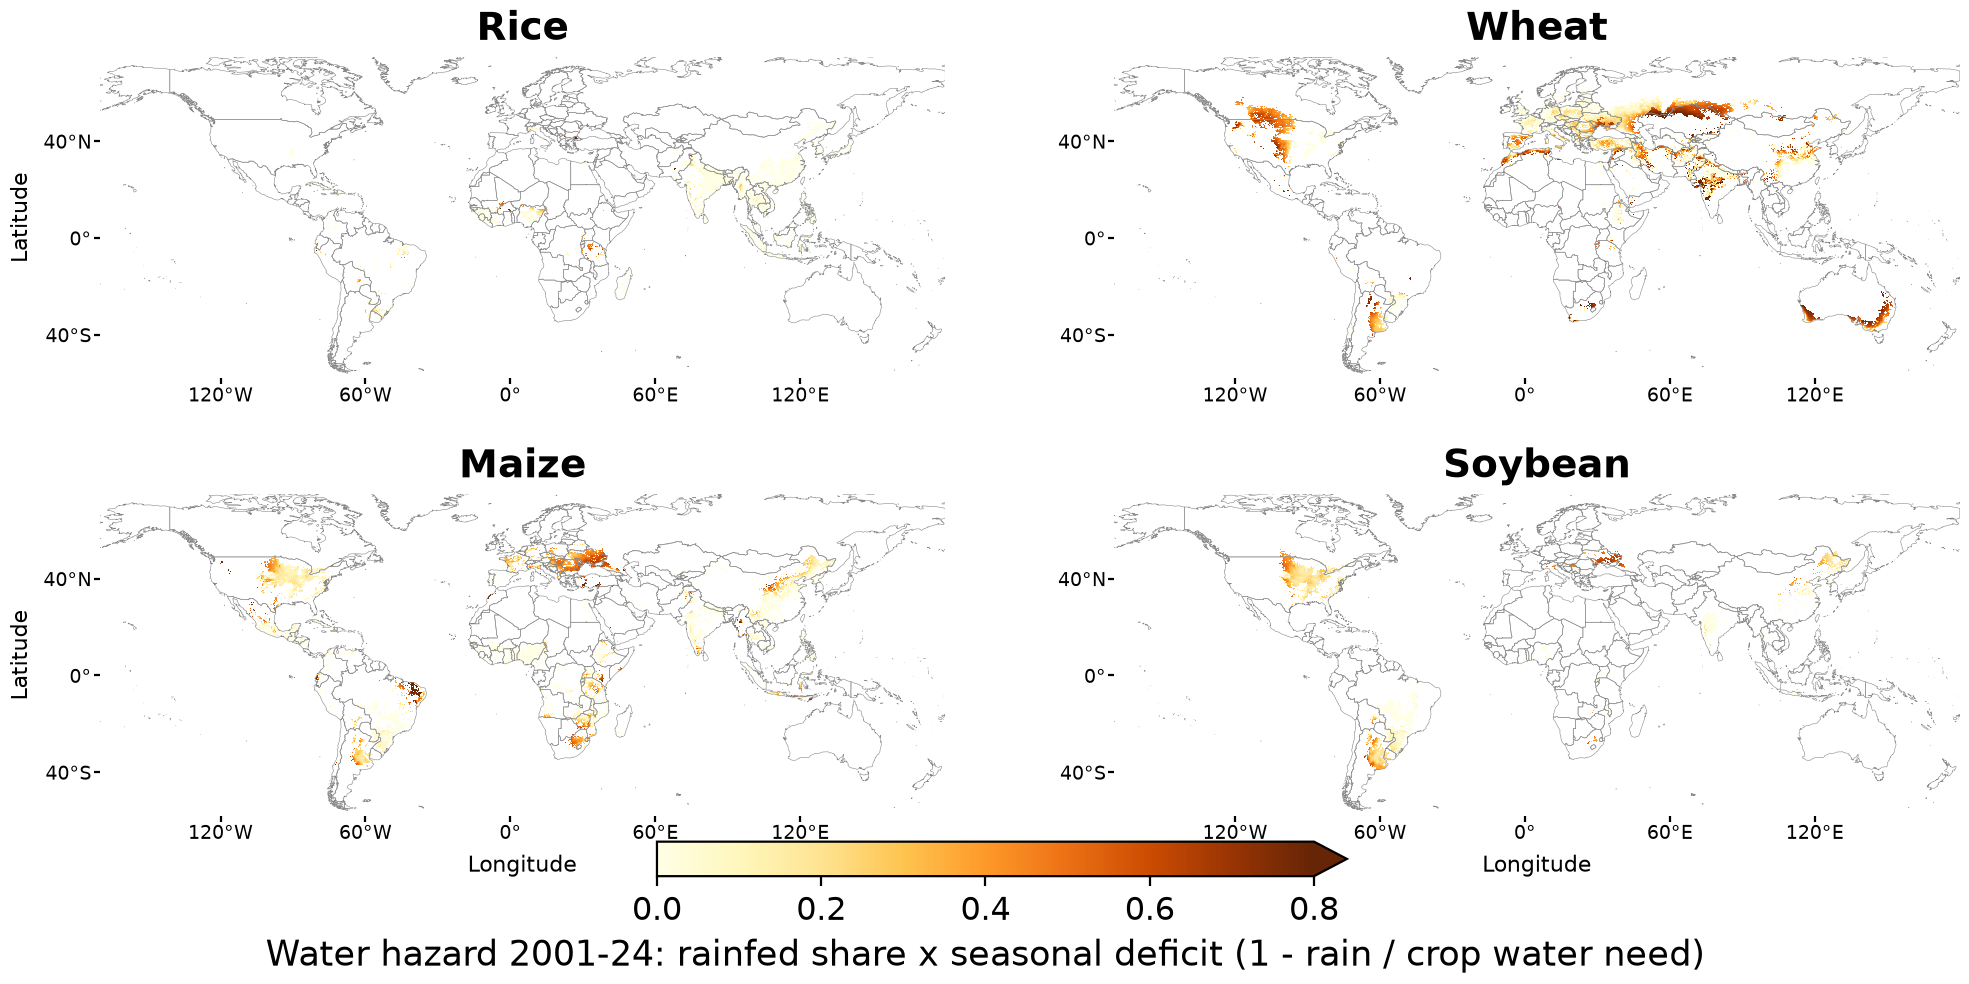
\includegraphics[width=0.95\linewidth,height=0.55\textheight,keepaspectratio]{F03_water_hazard_map.png}
\vspace*{0.2em}

\begin{columns}[T,onlytextwidth]
\column{0.48\textwidth}
\scriptsize
\textbf{What we measure:}\\
$\text{water stress} = \text{rainfed share} \times \max\!\big(0,\,1 - P/ET_c\big)$
\begin{itemize}\setlength{\itemsep}{0pt}
\item $P\ge ET_c$: zero shortfall; irrigated land: zero stress.
\end{itemize}
\column{0.48\textwidth}
\scriptsize
\textbf{Main finding \& why it matters:}
\begin{itemize}\setlength{\itemsep}{0pt}
\item Stress concentrates in dry, rainfed regions; irrigated rice/wheat show little.
\item Vulnerability depends not just on rainfall, but on crop reliance on rain.
\end{itemize}
\end{columns}
\end{frame}

\begin{frame}{Exposure by country}
\vspace*{-0.5em}
\centering
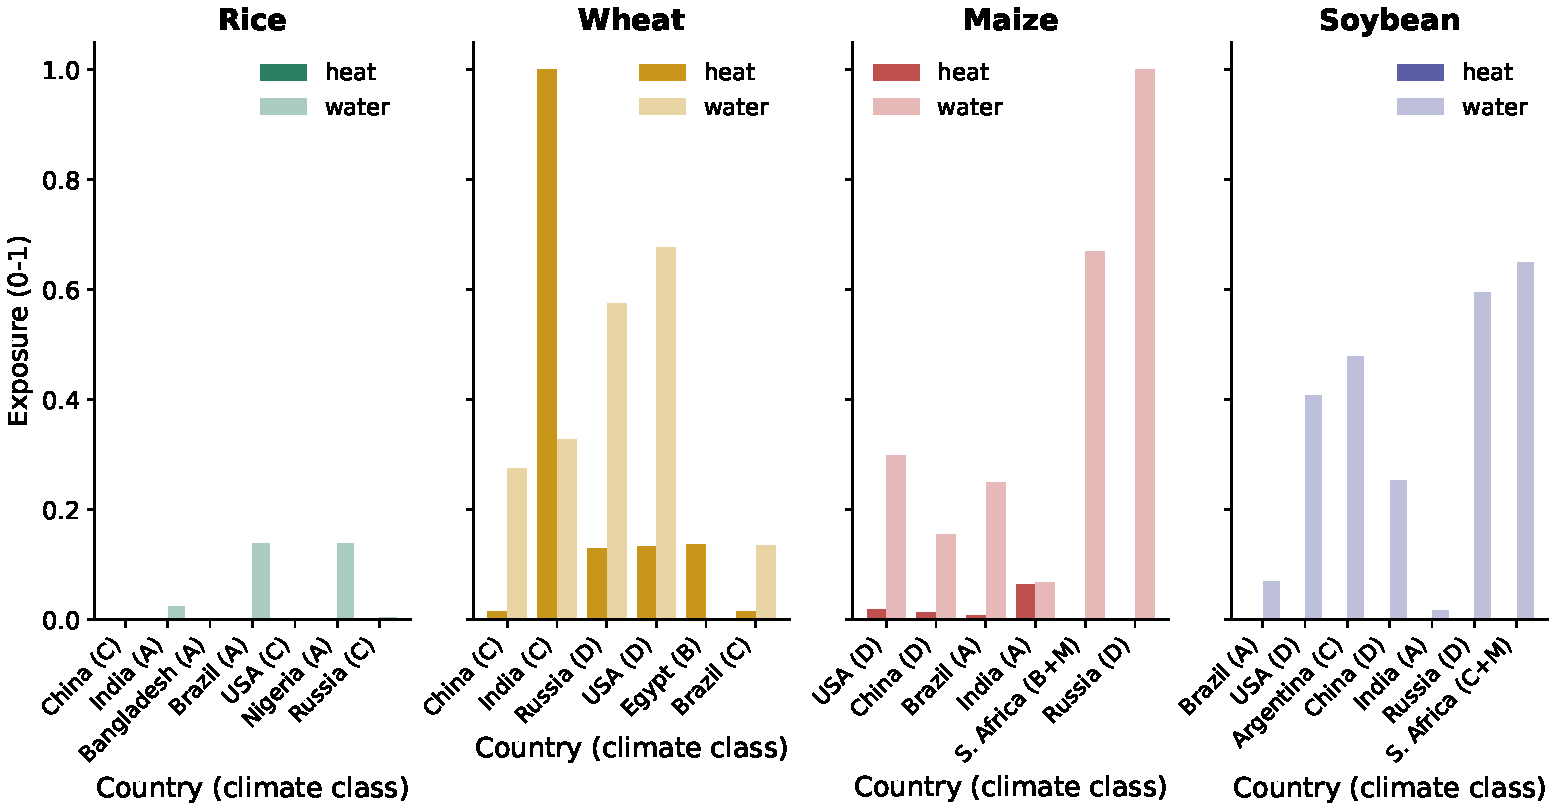
\includegraphics[width=0.92\linewidth,height=0.54\textheight,keepaspectratio]{F04_exposure_by_country.pdf}
\vspace*{0.1em}

\begin{columns}[T,onlytextwidth]
\column{0.32\textwidth}
\scriptsize
\textbf{Heat ($E^{\TT}$):}\\
Peaks for wheat in India (\exEheat) where flowering temperatures exceed \SI{25}{\celsius}.
\column{0.35\textwidth}
\scriptsize
\textbf{Water ($E^{\PP}$):}\\
Highest for maize in Russia/South Africa and wheat in USA/Russia (dry rainfed zones).
\column{0.29\textwidth}
\scriptsize
\textbf{Rice:}\\
Low on both: mostly irrigated and monthly means stay below its heat threshold.
\end{columns}
\end{frame}

\begin{frame}{Sensitivity by crop}
\vspace*{-0.5em}
\centering
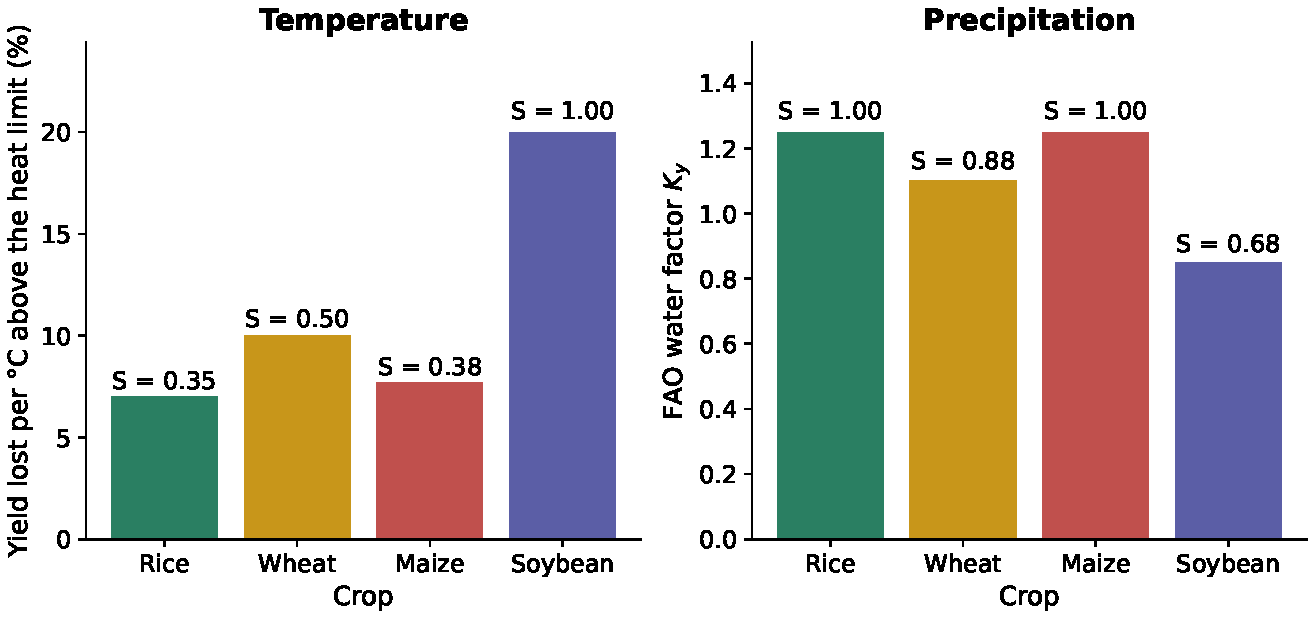
\includegraphics[width=0.88\linewidth,height=0.54\textheight,keepaspectratio]{F05l_literature_sensitivity.pdf}
\vspace*{0.1em}

\begin{columns}[T,onlytextwidth]
\column{0.32\textwidth}
\scriptsize
\textbf{Heat ($S^{\TT}$):}\\
Soybean is the most sensitive per \si{\celsius} above threshold, then wheat, maize, rice.
\column{0.33\textwidth}
\scriptsize
\textbf{Water ($S^{\PP}$):}\\
Rice and maize exhibit the highest FAO water factors ($K_y = 1.25$).
\column{0.31\textwidth}
\scriptsize
\textbf{One score per crop:}\\
Same literature values applied globally; sensitivity varies by crop, not country.
\end{columns}
\end{frame}

\begin{frame}{Importance and adequacy}
\begin{columns}[T]
\column{0.49\textwidth}
\centering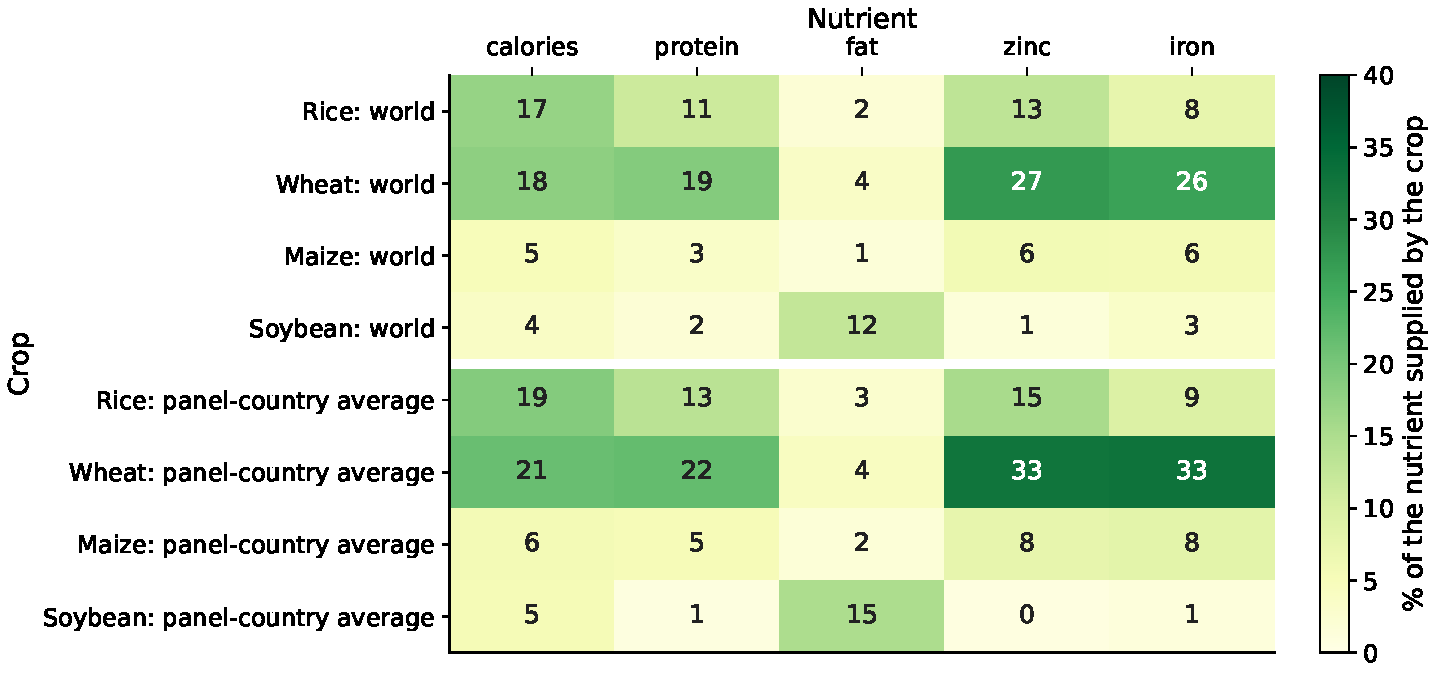
\includegraphics[width=\linewidth]{F06s_importance_summary.pdf}\\
\scriptsize \% of each nutrient supplied by the crop
\column{0.49\textwidth}
\centering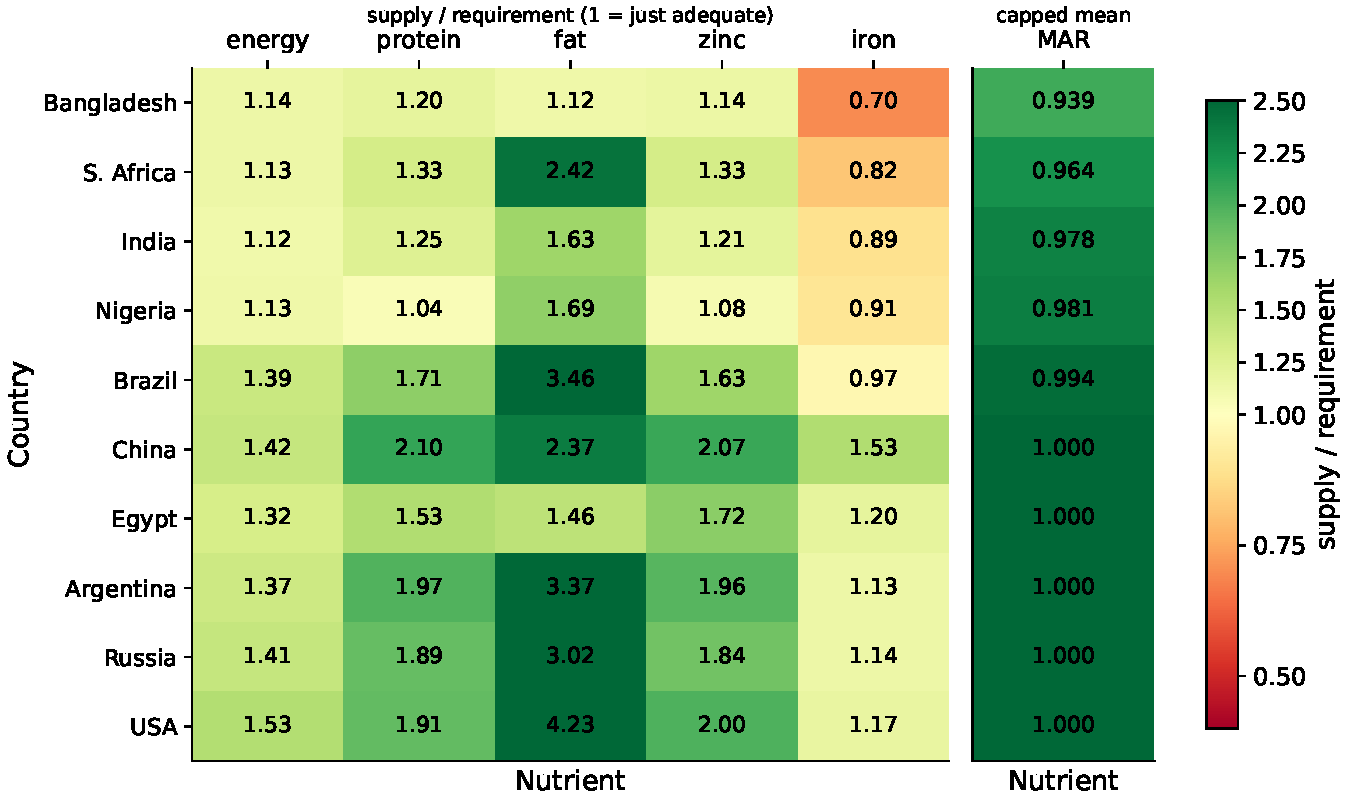
\includegraphics[width=\linewidth]{F07_adequacy_panel.pdf}\\
\scriptsize supply $\div$ requirement (1 = just enough)
\end{columns}
\par\vspace{0.3em}\footnotesize
\textbf{Result:} wheat and rice supply most protein, zinc and iron; soybean mainly fat (oil); maize little (mostly feed). \textbf{Iron is limiting}: supply $\div$ requirement \feRatioBangladesh\ (Bangladesh), \feRatioSAfrica\ (South Africa), \feRatioIndia\ (India); other nutrients are met. \textbf{Why it matters:} a yield loss in a crop people depend on, where a nutrient is already short, hurts nutrition most.
\end{frame}

\begin{frame}{Country-by-crop vulnerability index ($V_{F4}$)}
\begin{columns}[T]
\column{0.52\textwidth}
\centering
\adjustbox{max width=\linewidth}{\footnotesize\begin{tabular}{lcccc}
\toprule
\textbf{Country} & \textbf{Rice} & \textbf{Wheat} & \textbf{Maize} & \textbf{Soybean} \\
\midrule
USA & $<0.0001$ & 0.0747 & 0.0037 & 0.0197 \\
Brazil & 0.0039 & 0.0103 & 0.0103 & 0.0025 \\
India & 0.0023 & 0.1511 & 0.0015 & 0.0002 \\
China & 0.0001 & 0.0240 & 0.0016 & 0.0097 \\
Russia & $<0.0001$ & 0.1105 & 0.0021 & 0.0032 \\
Argentina & -- & -- & -- & 0.0052 \\
Bangladesh & 0.0002 & -- & -- & -- \\
Egypt & -- & 0.0209 & -- & -- \\
Nigeria & 0.0046 & -- & -- & -- \\
South Africa & -- & -- & 0.0895 & 0.0122 \\
\bottomrule
\end{tabular}
}
\column{0.46\textwidth}
\footnotesize
\textbf{Why values are on a small decimal scale:}\\
$V_{F4} = \tfrac12(E^{\TT}S^{\TT}+E^{\PP}S^{\PP})\,I$ multiplies three fractional shares ($\le 1$), yielding values from $10^{-5}$ to $0.15$.\\[0.4em]
\textbf{Key patterns:}
\begin{itemize}\setlength{\itemsep}{2pt}
\item \textbf{Wheat peaks:} in India ($0.1511$) and Russia ($0.1105$) from high dietary shares and climate exposure.
\item \textbf{Maize peaks:} in South Africa ($0.0895$) where it is a dietary staple on rainfed land.
\item \textbf{Rice stays low:} ($<0.005$) across all panel countries due to low observed heat exposure.
\end{itemize}
\end{columns}
\end{frame}

\begin{frame}{Result: the vulnerability index}
\begin{columns}[T]
\column{0.63\textwidth}
\centering
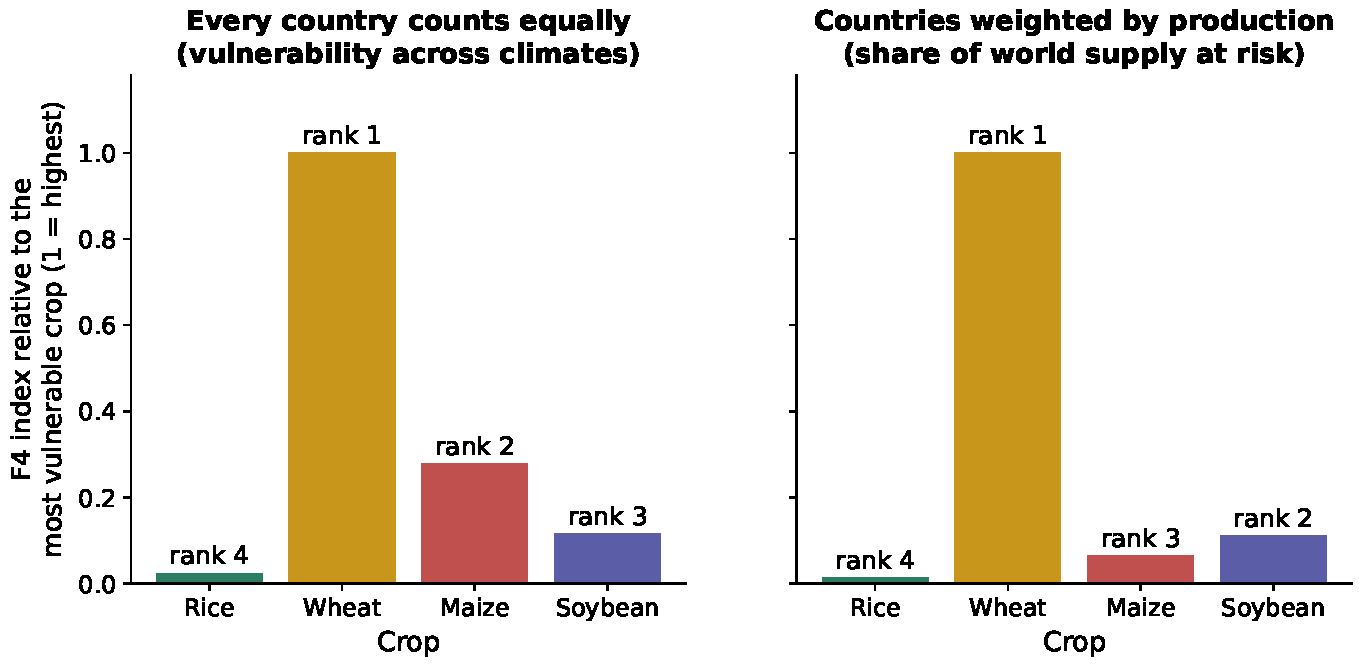
\includegraphics[width=\linewidth]{F08s_index_F4.pdf}
\column{0.35\textwidth}
\footnotesize
\textbf{Equal weights:} \orderFour\\ \textbf{Production-weighted:} \orderFourPw\\[0.4em]
Bar = index relative to the most vulnerable crop (= 1).\\[0.4em]
\textbf{Wheat (\#1 in both):} main source of protein, zinc, iron; exposed to heat in India and dry spells in USA/Russia.\\[0.4em]
\textbf{Rice (lowest in both):} mostly irrigated; monthly means stay below its \SI{35}{\celsius} limit.
\end{columns}
\end{frame}

\begin{frame}{Where does the vulnerability actually sit?}
\begin{columns}[T]
\column{0.60\textwidth}
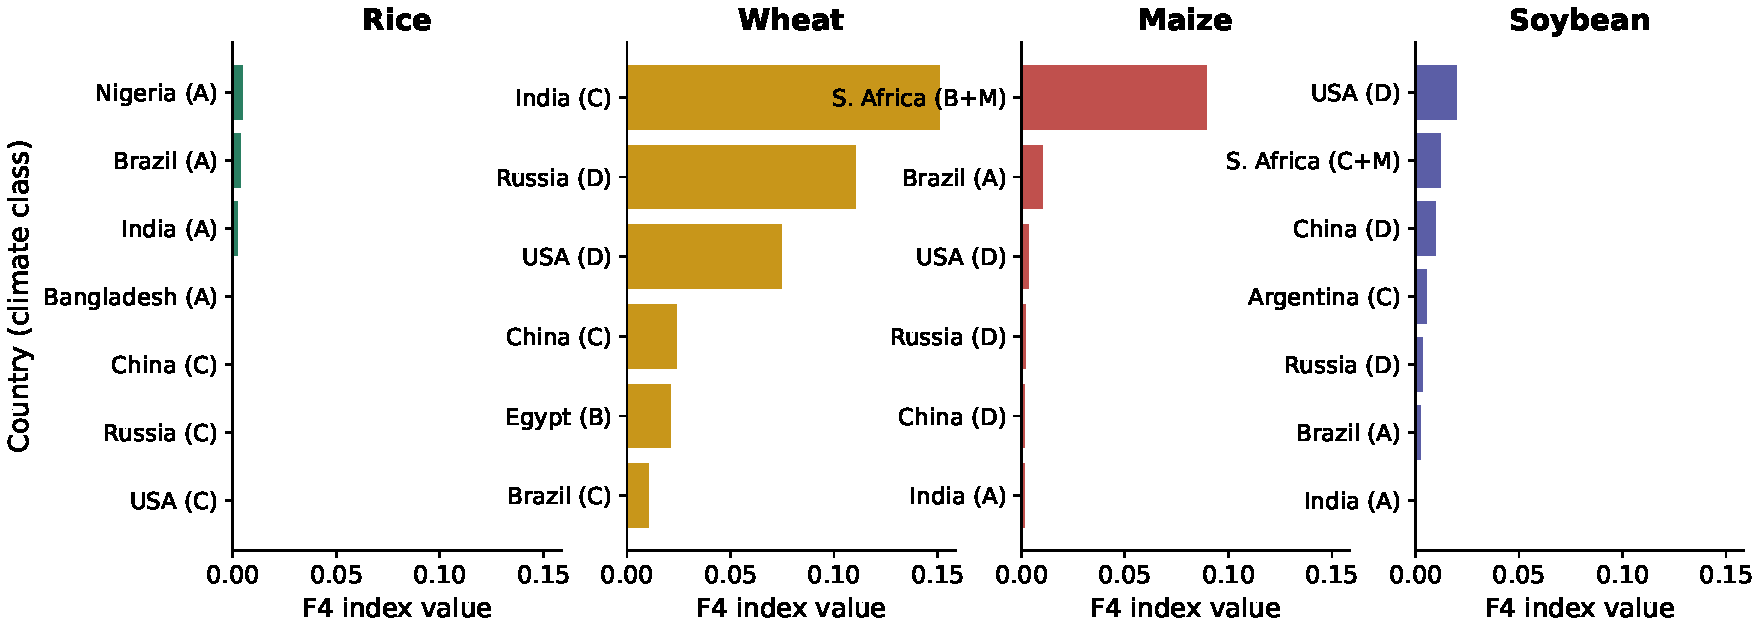
\includegraphics[width=\linewidth]{F09_country_index.pdf}
\column{0.38\textwidth}
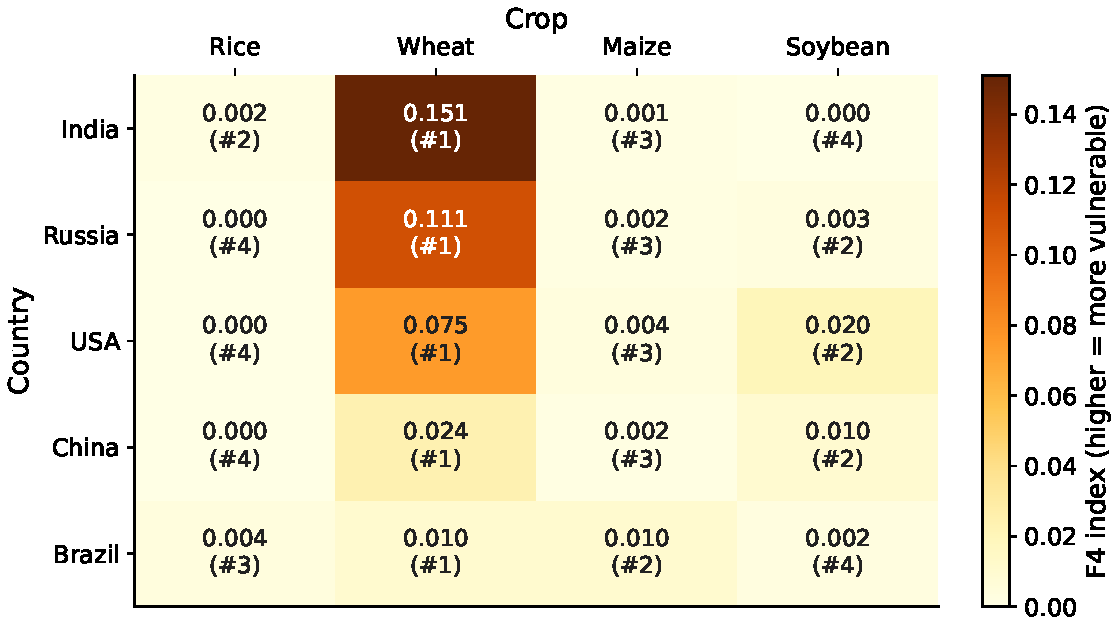
\includegraphics[width=\linewidth]{F17_country_crop_matrix.pdf}
\end{columns}
\par\footnotesize
Left figure: each bar is 1 country's index for a particular crop. Right figure: crops compared within the \nShared{} countries that grow all 4 crops (\#1 here means the most vulnerable crop there and so on...); wheat ranks \#1 in all \sharedWheatTop{} out of \nShared{} countries. Highest: wheat in India, Russia, USA; maize in South Africa.
\end{frame}

\begin{frame}{Yield to diet: results}
\begin{columns}[T]
\column{0.49\textwidth}
\centering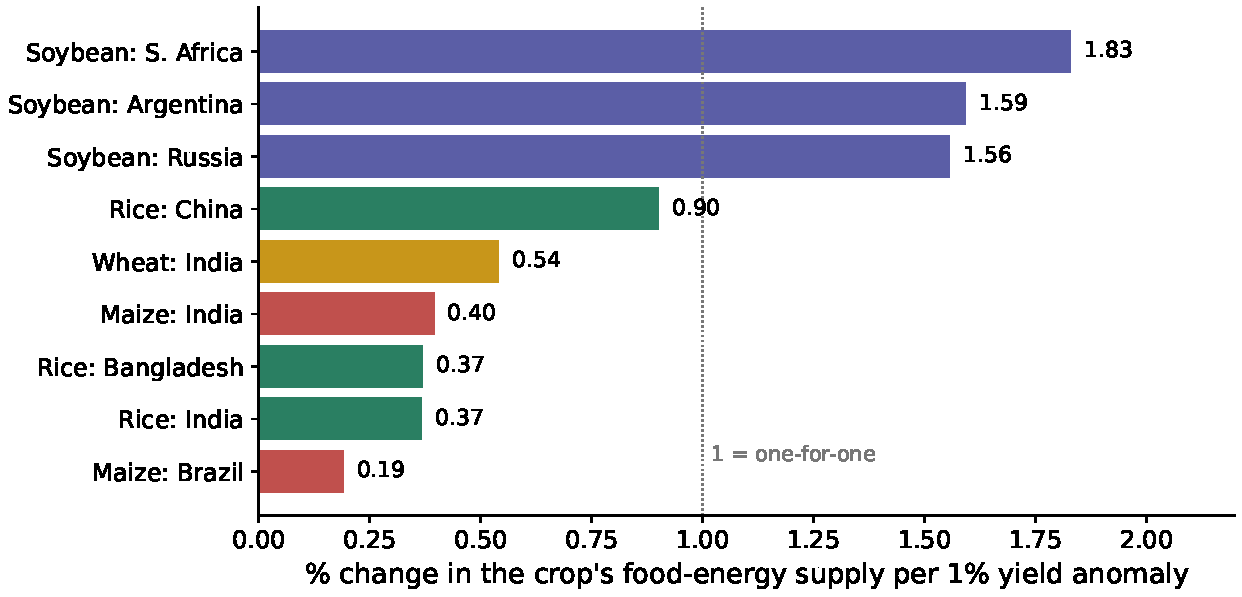
\includegraphics[width=\linewidth]{F13c_passthrough_clear.pdf}\\
\scriptsize pass-through $\beta$ (clear cases only)
\column{0.49\textwidth}
\centering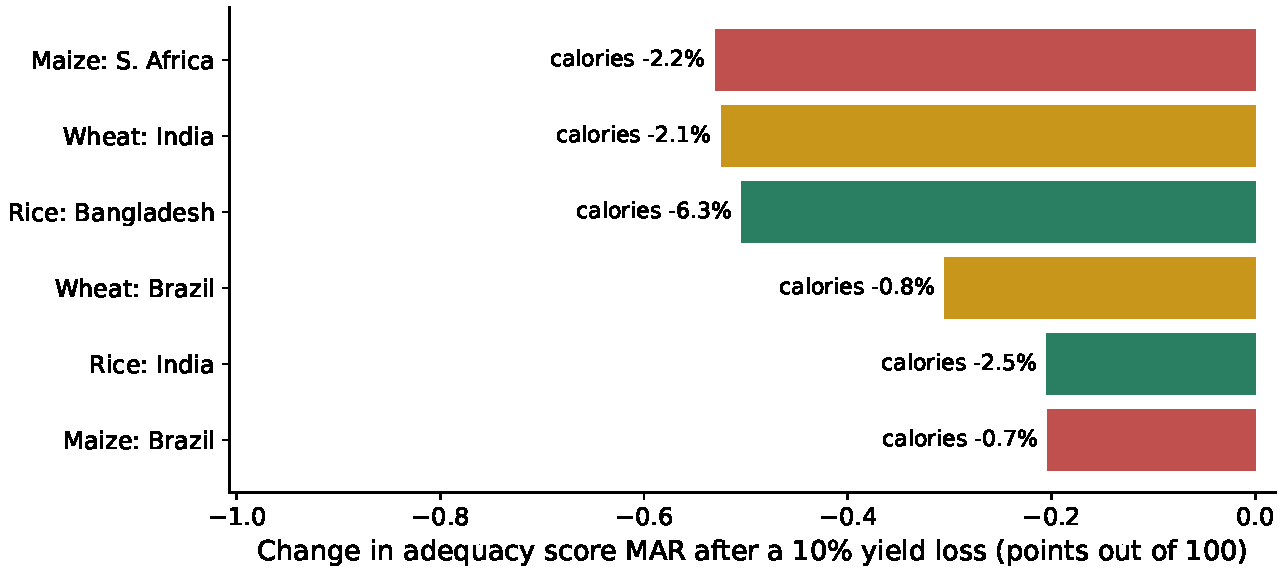
\includegraphics[width=\linewidth]{F14c_scenario_simple.pdf}\\
\scriptsize fall in MAR after a 10\% yield loss
\end{columns}
\par\vspace{0.3em}\footnotesize
Left figure: a bad harvest clearly lowers food supply in \nPassOldSig{} of \nPassOld{} cases, mainly rice in Asia and small soybean crops. Right figure: maize in South Africa and wheat in India lose most adequacy (they remove iron where it is short); rice in Bangladesh loses most calories (\bdShockKcalAbs\%). Exports can soften the loss (wheat in India: \inWheatMar\ $\rightarrow$ \inWheatMarTrade).
\end{frame}

% =====================================================================
\section{Conclusions}
\begin{frame}{Observations}
\small
\begin{enumerate}\setlength{\itemsep}{4pt}
\item \textbf{Wheat is the most vulnerable crop:} \orderFour\ (equal weights).
\item \textbf{Why wheat:} importance and exposure. Maize and soybean are the most heat-sensitive (\poolTMaize\% and \poolTSoybean\% yield per \si{\celsius}; wheat \poolTWheat\%) but little is eaten directly.
\item \textbf{Most vulnerable pairs:} wheat in India, Russia, USA; maize in South Africa.
\item \textbf{Iron} is the nutrient closest to running short.
\item \textbf{Rice scores lowest because of the measure, not proof of safety:} mostly irrigated, and monthly means stay below its \SI{35}{\celsius} limit though short heat spikes can still harm flowering. Where rice is the staple (Bangladesh: \bdRiceKcal\% of calories) an underestimate would matter.
\end{enumerate}
\end{frame}

\begin{frame}{Data used}
\small
\begin{tabular}{p{4.0cm}p{5.8cm}p{3.0cm}}
\toprule
Dataset & What it gives & Index term\\
\midrule
WorldClim 2.1 & monthly Tmax, Tmin, rainfall & Exposure\\
SPAM 2010 & where each crop grows; irrigated vs rainfed & Exposure\\
Sacks crop calendar & planting and harvest dates & Exposure\\
FAOSTAT crops & production, area, yield & Countries, Sensitivity\\
FAO Food Balance Sheets & food supply of calories, protein, fat, each food & Importance\\
USDA FoodData Central & zinc and iron per food & Importance\\
FAO energy requirement & average requirement per person & Adequacy\\
\bottomrule
\end{tabular}
\end{frame}

\begin{frame}[allowframebreaks]{References}
\renewcommand{\bibsection}{}
\scriptsize
\bibliography{refs}
\end{frame}

\end{document}


